\documentclass{standalone}
\usepackage{tikz}
\usetikzlibrary{arrows.meta, positioning, shapes.geometric}

\begin{document}
	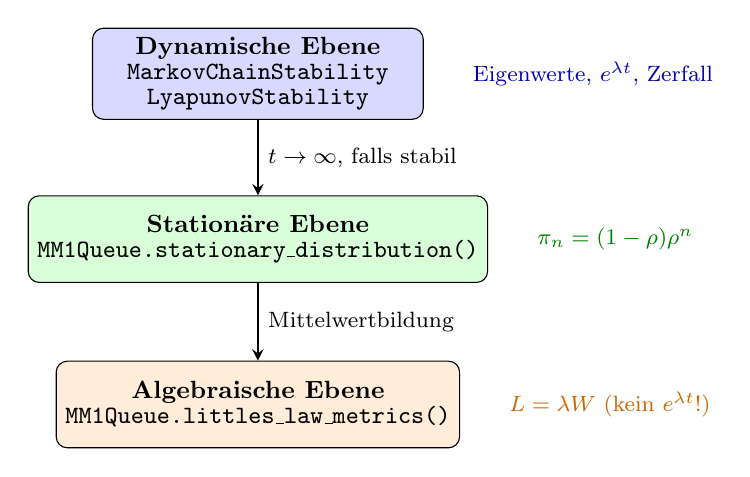
\begin{tikzpicture}[
		box/.style={draw, rounded corners, minimum width=4.2cm,
			minimum height=1.1cm, align=center, font=\small},
		arrow/.style={->, thick, >=stealth}
		]
		\node[box, fill=blue!15]   (dyn)  at (0,4.2)
		{\textbf{Dynamische Ebene}\\[-2pt]
			\texttt{MarkovChainStability}\\[-2pt]
			\texttt{LyapunovStability}};
		\node[box, fill=green!15]  (stat) at (0,2.1)
		{\textbf{Stationäre Ebene}\\[-2pt]
			\texttt{MM1Queue.stationary\_distribution()}};
		\node[box, fill=orange!15] (alg)  at (0,0)
		{\textbf{Algebraische Ebene}\\[-2pt]
			\texttt{MM1Queue.littles\_law\_metrics()}};
		\draw[arrow] (dyn)  -- node[right, font=\footnotesize]
		{$t\to\infty$, falls stabil} (stat);
		\draw[arrow] (stat) -- node[right, font=\footnotesize]
		{Mittelwertbildung} (alg);
		\node[right=0.5cm of dyn,  font=\footnotesize, text=blue!70!black]
		{Eigenwerte, $e^{\lambda t}$, Zerfall};
		\node[right=0.5cm of stat, font=\footnotesize, text=green!50!black]
		{$\pi_n = (1-\rho)\rho^n$};
		\node[right=0.5cm of alg,  font=\footnotesize, text=orange!80!black]
		{$L=\lambda W$ (kein $e^{\lambda t}$!)};
	\end{tikzpicture}
\end{document}